\documentclass[11pt,a4paper]{article}
\usepackage[T1]{fontenc}\usepackage[utf8]{inputenc}
\usepackage{lmodern,microtype,amsmath,amssymb,amsthm,mathtools}
\usepackage{booktabs,longtable,array,enumitem,xcolor,geometry,fancyhdr,hyperref,graphicx}
\geometry{margin=22mm}
\hypersetup{colorlinks=true,linkcolor=blue!55!black,urlcolor=blue,citecolor=blue!55!black,
 pdftitle={FIN ST1542--ST1631: Noncirculant Robustness, Continuum Minimax, Continuous Prior and Fiber Identifiability},
 pdfauthor={Krzysztof Żuchowski}}
\pagestyle{fancy}\fancyhf{}\fancyhead[L]{FIN ST1542--ST1631}\fancyhead[R]{Release 11.01}\fancyfoot[C]{\thepage}\setlength{\headheight}{14pt}
\newtheorem{theorem}{Theorem}\newcommand{\status}[1]{\textsf{[#1]}}

\begin{document}
\begin{titlepage}\centering\vspace*{14mm}
{\Huge\bfseries FIN ST1542--ST1631\par}\vspace{4mm}
{\LARGE Noncirculant Robustness, Continuum Minimax,\par}\vspace{2mm}
{\LARGE Continuous Prior and Fiber Identifiability\par}\vspace{12mm}
{\Large Krzysztof \.Zuchowski\par}
{\normalsize Independent Researcher --- Fractal Information Theory Project\par}
{\normalsize ORCID: 0009-0002-0909-3613\par}\vspace{9mm}
{\large Six research rounds --- 90 programmes\par}
{\large Release 11.01 --- 31 August 2026\par}
\vfill
\begin{minipage}{.87\textwidth}\small
This report extends the conditional FIN Operational/State discriminator beyond
circulant rounding errors and finite nuisance grids.  It proves noncirculant
operator-norm location robustness, brackets the continuous minimax value,
constructs a continuous-prior e-process theorem, certifies independent
calibration maps and resolves fine-fiber identifiability on a declared range.
\end{minipage}\vfill
{\small English mathematical and computational research report.}
\end{titlepage}

\begin{abstract}
ST1542--ST1631 extend the Release 11.00 robustness ladder in five directions.
First, Duhamel estimates remove the circulant requirement for the base return-
gap location.  If $A$ and $B$ are self-adjoint positive semidefinite graph
Laplacians with $\|B-A\|\le\epsilon$, then heat and unitary propagators differ
by at most $t\epsilon$ in operator norm.  Classical return changes by at most
$t\epsilon$, quantum return by at most $2t\epsilon$, and their gap by at most
$3t\epsilon$.  Combining this with the certified outside margin proves that
every global maximizer remains in $[0.59,0.60]$ whenever
\[
\epsilon<9.720652006795929\times10^{-8}.
\]
The bound does not preserve uniqueness inside that interval and does not cover
non-positive heat generators or dephasing-generator sensitivity.

Second, the continuous bidirectional-KL minimax value is certified.  A finite
LP proposes endpoint weights near $(0.318,0,0,0.682)$.  An adaptive outward
cover proves that this candidate achieves at least $0.05$ over the entire
$(\alpha,\gamma)$ rectangle.  A fixed two-point dual nuisance measure proves
that no allocation can exceed $0.05370588868619479$.  Therefore
\[
0.05\le V_*\le0.05370588868619479.
\]
The exact optimizer remains open.

Third, for a uniform continuous prior over the nuisance rectangle, the integral
of pointwise likelihood-ratio martingales is itself a nonnegative mean-one
martingale by Tonelli/Fubini.  It yields a valid one-sided anytime test.  A
positive $7\times9$ Gauss--Legendre rule supplies an executable 63-component
finite mixture which is valid independently of its quadrature accuracy; it is
not claimed to equal the exact continuous integral.

Fourth, independent classical and quantum calibration maps with up to five
percent uniform preparation contamination and two percent false-positive/
false-negative rates are certified directly rather than by a crude triangle
bound.  The base return ranges remain disjoint, and a complete 1000-cell
composite cover gives
\[
\mathrm{RSS}\ge0.022937735365240054.
\]

Finally, fine-fiber coupling $q$ is analysed.  Heat return
$(1+e^{-2qt})/2$ globally identifies $q\ge0$ from one nontrivial time.  Quantum
return $\cos^2(qt)$ is globally aliased but injective on its first monotone
branch.  At one time the two channels cross repeatedly.  The two-time design
$(0.6,1.0)$ has an interval-certified separation on $q\in[0.1,2]$:
\[
\mathrm{RSS}\ge0.009270580748993435.
\]
At $q=0$ both returns equal one for all times, giving an exact obstruction.

Protocol 11.01 freezes these claims and their boundaries.  No platform,
physical calibration, state ontology or natural event record is supplied.
\end{abstract}

\tableofcontents\newpage

\section{Round I: ST1542--ST1556 --- noncirculant Duhamel bounds}

Let $A$ and $B$ be positive semidefinite self-adjoint graph Laplacians with
zero row sums and
\[
\|B-A\|\le\epsilon.
\]
No circulant symmetry or shared eigenvectors are assumed.

For heat semigroups, Duhamel's formula gives
\[
e^{-tB}-e^{-tA}
=-\int_0^t e^{-(t-s)B}(B-A)e^{-sA}\,ds.
\]
Both semigroups are contractions, hence
\[
\|e^{-tB}-e^{-tA}\|\le t\epsilon.
\]
The unitary analogue gives the same bound:
\[
\|e^{-itB}-e^{-itA}\|\le t\epsilon.
\]

For the selected return effect,
\[
|C_B(t)-C_A(t)|\le t\epsilon,
\qquad
|Q_B(t)-Q_A(t)|\le2t\epsilon,
\]
and therefore
\[
|D_B(t)-D_A(t)|\le3t\epsilon.
\]

Let $t_c=0.5945308$ and let
$m=3.089572412462438\times10^{-6}$ be the certified gap between the candidate
value and every point outside $[0.59,0.60]$.  For $t\le10$,
\[
D_B(t_c)-D_B(t)
\ge m-3(t_c+10)\epsilon.
\]
Hence all global maximizers of $D_B$ remain in $[0.59,0.60]$ if
\[
\boxed{\epsilon<9.720652006795929\times10^{-8}.}
\]

For arbitrary symmetric entrywise errors bounded by $\delta$, the crude
$\|E\|\le12\delta$ condition gives
$\delta<8.100543338996607\times10^{-9}$ as sufficient.  At
$\epsilon=10^{-8}$ the exclusion margin remains
$2.771736488462438\times10^{-6}$.

\begin{theorem}[noncirculant location robustness]
Within the declared graph-Laplacian norm ball, every global return-gap
maximizer remains in $[0.59,0.60]$ below the stated threshold.
\end{theorem}

The theorem does not guarantee a unique critical point after noncirculant
perturbation.  It also does not propagate uncertainty through the dephasing
Lindbladian.

\section{Round II: ST1557--ST1571 --- continuous minimax value}

For the four scheduled times define
\[
d_i(\theta)=\min\{D(C_i\|Q_{i,\theta}),D(Q_{i,\theta}\|C_i)\},
\]
and
\[
V_*=\sup_{w\in\Delta_3}\inf_{\theta\in[0.9,1.1]\times[0,100]}
\sum_iw_id_i(\theta).
\]

A $41\times401$ grid LP produces a two-endpoint candidate.  Its exact displayed
weights depend slightly on grid resolution, so only the structural conclusion
is retained: roughly $32\%$ at $t=0.3$ and $68\%$ at $t=2.0$.

For an interval $q\in[q_-,q_+]$, Bernoulli KL is jointly convex and minimized
at $q=p$ if the probability intervals overlap, otherwise at the nearest
endpoints.  This analytic rectangle minimum, combined with outward return
intervals, permits adaptive subdivision of the continuous nuisance rectangle.
Starting from 1000 cells, 380 splits produce 1380 accepted boxes and prove the
candidate value is at least $0.05$.

For the converse, take nuisance points $(1.1,16)$ and $(1.1,16.25)$ with weights
$0.7622353358$ and $0.2377646642$.  For any time allocation, its worst-case
value cannot exceed the weighted average over these two points, whose largest
time coordinate is $0.053705888685\ldots$; a rounding safety payment yields
the upper bound $0.05370588868619479$.

\begin{theorem}[continuous minimax value bracket]
For the frozen decimal model, declared times, nuisance rectangle and
bidirectional-KL metric,
\[
\boxed{0.05\le V_*\le0.05370588868619479.}
\]
\end{theorem}

The theorem proves near-optimality in value, not exact weights or a unique
active nuisance measure.

\section{Round III: ST1572--ST1586 --- continuous-prior e-process}

Let $\pi$ be the uniform probability measure on
$[0.9,1.1]\times[0,100]$.  For every nuisance point $\theta$, define
\[
L_{\theta,n}=\prod_{i=1}^n
\frac{q_\theta(X_i|t_i)}{p_C(X_i|t_i)}.
\]
Under the classical null, $L_{\theta,n}$ is a nonnegative mean-one martingale.
Tonelli/Fubini therefore gives
\[
E_n^{\rm cont}=\int L_{\theta,n}\,\pi(d\theta),
\qquad
\mathbb E_C E_n^{\rm cont}=1.
\]

\begin{theorem}[continuous-prior anytime rejection]
\[
\Pr_C\left(\sup_nE_n^{\rm cont}\ge100\right)\le0.01.
\]
\end{theorem}

The executable approximation uses positive Gauss--Legendre weights with seven
clock nodes and nine dephasing nodes.  Their 63-component convex sum is itself
a valid finite-mixture e-process regardless of quadrature accuracy.  It is not
the exact integral.  A synthetic off-node alternative
$(\alpha,\gamma)=(1.03,7.3)$ crossed after 243 events; this is a power fixture,
not evidence or a uniform stopping guarantee.

Both the exact prior integral and the finite quadrature mixture are one-sided
tools for rejecting $C$.  They do not uniformly accept $C$ against all
quantum nuisance values.

\section{Round IV: ST1587--ST1601 --- independent calibration}

Each hypothesis receives an independent affine map
\[
T_{\epsilon,a,b}(p)
=a+(1-a-b)\left[(1-\epsilon)p+\epsilon/12\right],
\]
with
\[
0\le\epsilon\le0.05,qquad0\le a,b\le0.02.
\]
Because the map is multiaffine in $(\epsilon,a,b)$ and monotone in $p$, extrema
occur at the eight calibration vertices.

At $t=0.6$, the independently calibrated ranges are
\[
C_{\rm obs}\in[0.3879880701,0.4241102492],
\]
\[
Q_{\rm obs}\in[0.7708322380,0.8271041102].
\]
They remain separated by at least $0.3467219888$.

The same vertex range construction is applied to every cell of the complete
1000-cell $(\alpha,\gamma)$ cover.  It yields
\[
\boxed{\mathrm{RSS}_{\rm independent}\ge0.022937735365240054,}
\]
so at least one calibrated time differs by
$0.07572604466965123$.

This upgrades the earlier $5\%+2\%$ status.  The old triangle bound failed to
certify the box because it ignored the affine geometry; that failure was not a
counterexample.  The present theorem is still limited to binary affine
calibration.  Vertex-dependent detector matrices remain open.

Independent uniform click efficiencies in $[0.8,1]$ do not alter
click-conditioned ranges, but attempts and no-clicks remain mandatory.

\section{Round V: ST1602--ST1616 --- fine-fiber $q$}

For initial fiber state zero,
\[
H_q(t)=\frac{1+e^{-2qt}}2,
\qquad
R_q(t)=\cos^2(qt).
\]

For every $t>0$, $H_q$ is strictly decreasing on $q\ge0$ and
\[
q=-\frac{\log(2H-1)}{2t}.
\]
Thus classical $q$ is globally identifiable from one nontrivial return.

Quantum return has aliases
\[
q'=\frac{k\pi}{t}\pm q.
\]
It is injective only on a specified monotone branch, for example
\[
0\le q\le\frac{\pi}{2t},qquad
q=\frac{\arccos\sqrt R}{t}.
\]

At $q=0.37$, $t=0.6$,
\[
H=0.8207327104,qquad R=0.9515203359,qquad R-H=0.1307876255.
\]
The ideal Bernoulli Fisher informations are approximately $1.006807$ for heat
and $4t^2=1.44$ for the quantum branch.

One time does not always distinguish the channels: at $t=0.6$ their positive
crossings below $10$ occur near $1.07725$, $3.93441$, $6.54466$ and $9.16299$.
Moreover,
\[
H_0(t)=R_0(t)=1
\]
for every time, so $q=0$ is an exact no-go.

For $q\in[0.1,2]$, a 1900-box outward interval cover at times $(0.6,1.0)$ proves
\[
\boxed{
(R_q(0.6)-H_q(0.6))^2+
(R_q(1)-H_q(1))^2
\ge0.009270580748993435.}
\]
At least one residual is at least $0.06808296684558274$.

The result is conditional on the $q$ range, clock and fiber-resolving
instrument.  It does not derive a physical $q$.

\begin{figure}[ht]
\centering
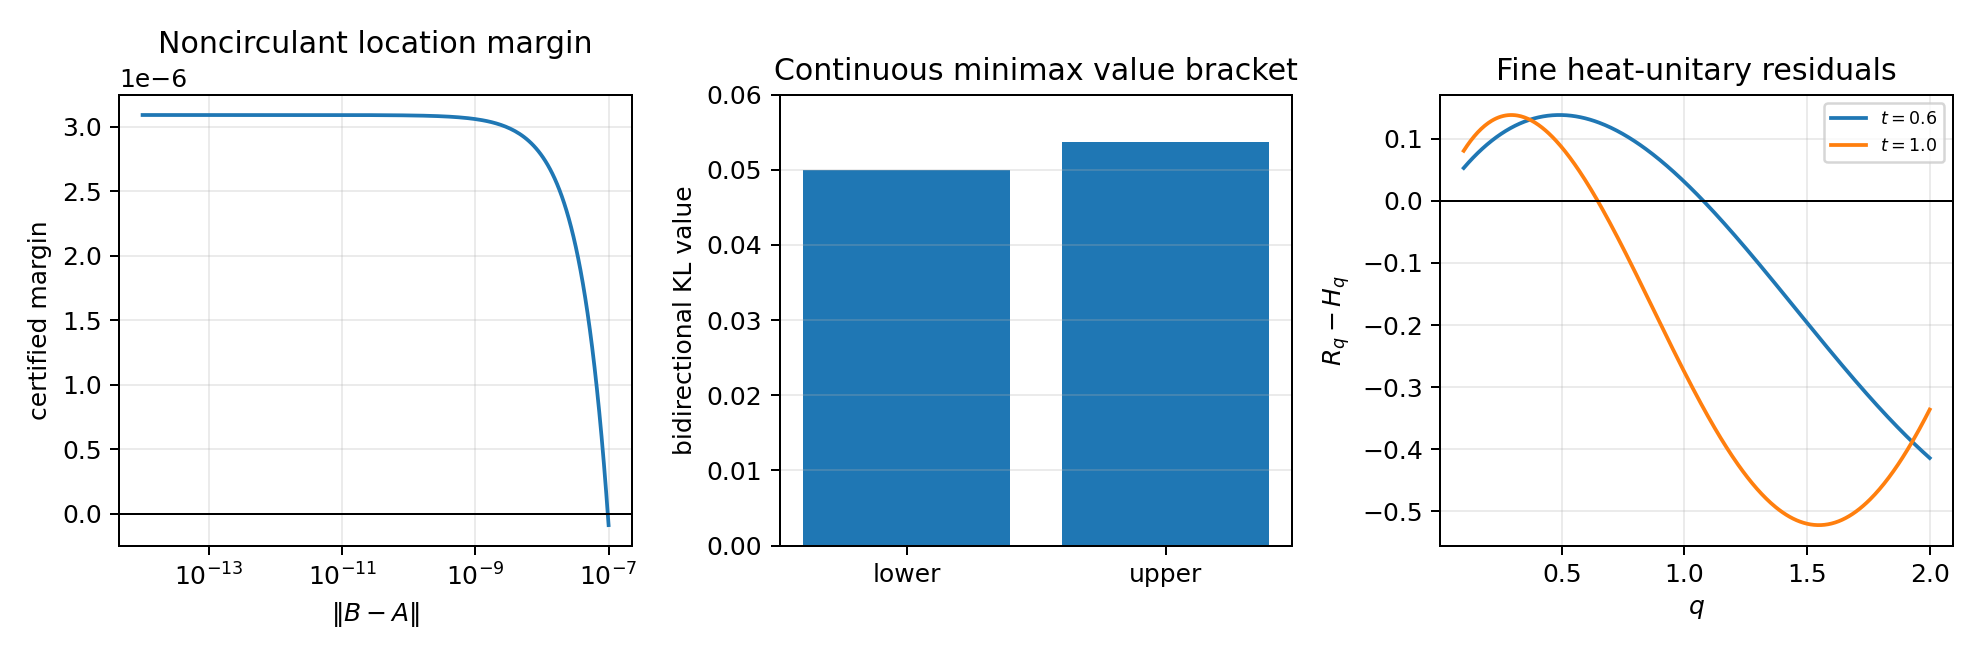
\includegraphics[width=.98\textwidth]{FIN_ST1542_ST1631_Figures/continuum_and_fiber_summary.png}
\caption{Left: noncirculant location margin versus operator perturbation.
Centre: certified continuous minimax value bracket.  Right: the two fine-fiber
heat--unitary residuals over the certified $q$ range.}
\end{figure}

\section{Round VI: ST1617--ST1631 --- synthesis}

\begin{longtable}{@{}p{.34\textwidth}p{.21\textwidth}p{.35\textwidth}@{}}
\toprule
Result & Status & Boundary \\
\midrule\endhead
noncirculant maximum location & \status{Proven bound} & PSD graph Laplacians, norm threshold \\
continuous minimax value & \status{Certified bracket} & frozen metric/model \\
exact continuous-prior e-process & \status{Proven} & one-sided classical-null rejection \\
63-node quadrature e-process & \status{Executable/proven finite} & not exact integral \\
independent calibration RSS & \status{Interval-proven} & binary affine maps \\
classical $q$ inversion & \status{Proven} & known heat channel \\
quantum $q$ branch inversion & \status{Proven conditional} & specified alias-free range \\
two-time fine channel separation & \status{Interval-proven} & $q\in[0.1,2]$ \\
platform/evidence & \status{Absent} & no external calibration/events \\
\bottomrule
\end{longtable}

Protocol \path{FIN_ST1617_ST1631_Protocol_11_01.json} hashes Release 11.00,
the continuous-prior quadrature and the independent calibration polytope, and
records the noncirculant threshold, minimax bracket and fine-fiber range.

The robustness hierarchy now includes decimal, circulant, noncirculant,
continuous-nuisance, independent-calibration and exact-refinement/fine-fiber
layers.  It still describes one conditional $OA$, not strict FIN physics.

The experiment tests internal channel/fiber dynamics.  It does not test literal
nonexistence of the whole nadsoliton.

\section{Recommended next programmes}

\begin{enumerate}
\item derive Duhamel bounds for the full dephasing/Lindblad generator;
\item propagate symbolic $(\omega,\phi,\beta,\eta)$ interval uncertainty;
\item isolate exact minimax weights through KKT/dual equations;
\item construct uniformly valid composite acceptance or confidence sets;
\item certify a vertex-dependent detector matrix polytope;
\item jointly identify fiber $q$ and clock scale;
\item impose multi-level $q$ consistency;
\item optimize the continuous prior for power while preserving validity;
\item derive one platform-specific transfer function;
\item freeze an external calibration form;
\item obtain independent audit;
\item collect raw events only after every preceding freeze.
\end{enumerate}

Stop if location robustness is called uniqueness, a value bracket is called an
exact optimizer, quadrature is called exact integration, an affine detector is
called an arbitrary matrix, the $q$ theorem is applied at $q=0$ or outside its
range, or synthetic power is called evidence.

\section{Final conclusion}

\begin{quote}
The conditional FIN dual-dynamics protocol now has a noncirculant operator-norm
location theorem, a certified continuous minimax value, an exact continuous-
prior anytime theorem, a positive independent-calibration certificate and an
interval-certified fine-fiber test.  The remaining obstacles are no longer
ordinary finite numerical ambiguity; they are full generator uncertainty,
general detector matrices, exact composite decisions and physical realization.
\end{quote}

\appendix
\section{Six-round ledger}
\begin{longtable}{@{}p{.18\textwidth}p{.34\textwidth}p{.38\textwidth}@{}}
\toprule
Range & Object & Verdict \\
\midrule\endhead
ST1542--ST1556 & noncirculant perturbation & global location bound \\
ST1557--ST1571 & continuous minimax & value bracket $[0.05,0.053706]$ \\
ST1572--ST1586 & continuous-prior e-process & exact theorem, finite quadrature \\
ST1587--ST1601 & independent calibration & positive base and composite separation \\
ST1602--ST1616 & fine-fiber $q$ & inversion/aliasing/two-time certificate \\
ST1617--ST1631 & synthesis & six-layer conditional robustness hierarchy \\
\bottomrule
\end{longtable}

\section{Reproducibility}
The authoritative result sets run from
\path{FIN_ST1542_ST1556_Results.json} through
\path{FIN_ST1617_ST1631_Results.json}.  Each contains fifteen programmes and
packet SHA-256 references.  The combined test
\path{test_fin_st1542_st1631.py} verifies all ninety packets, perturbation
thresholds, continuous bracket, prior grid, independent calibration, fiber
certificate, protocol, figure and nonpromotion gates.

\section{Nonclaims}
No noncirculant dephasing uncertainty theorem, exact minimax weights, symmetric
composite decision, arbitrary detector matrix certificate, physical $q$ source,
state ontology, platform, raw event, independent custody, legacy bridge,
selector, Standard Model, gravity, $L_{\rm total}$ or Theory of Everything is
established.  All future FIN PDFs remain English.

\begin{thebibliography}{9}
\bibitem{engel} K.-J. Engel and R. Nagel, \emph{One-Parameter Semigroups for Linear Evolution Equations}, Springer.
\bibitem{moore} R. E. Moore, R. B. Kearfott and M. J. Cloud, \emph{Introduction to Interval Analysis}, SIAM.
\bibitem{ville} J. Ville, \emph{Etude critique de la notion de collectif}, Gauthier-Villars.
\end{thebibliography}
\end{document}
